\documentclass[serif,mathserif]{beamer}
\usepackage{amsmath, amsfonts, epsfig, xspace}
\usepackage{algorithm,algorithmic}
\usepackage{pstricks,pst-node}
\usepackage{multimedia}
\usepackage[normal,tight,center]{subfigure}
\setlength{\subfigcapskip}{-.5em}
\usepackage{beamerthemesplit}
\usetheme{lankton-keynote}

\author[Mosca]{ Just another Simple static analysis tool to find bugs like a grep unix command \quad 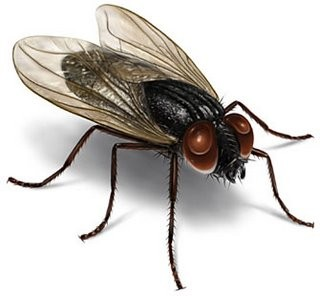
\includegraphics[width=3cm]{images/mosca.jpg} }

\title[ Page \hspace{2em}\insertframenumber/\inserttotalframenumber]{Mosca}

\date{February 8, 2015} 

\institute{Antonio Costa - CoolerVoid - coolerlair[aT]gmail[DOt]com}

\begin{document}

\maketitle

% \section{Introduction}  % add these to see outline in slides



\begin{frame}
  \frametitle{Whoami}
  Author:
  \begin{itemize}  \item  Antonio Costa "CoolerVoid" is a Computer Programmer who loves the Hacker culture, he work as system analyst at CONVISO for three years. Nowadays, Antonio working with code review, pentest and security research with focus on Secure Web Applications and Reverse Engineering and he has speaking in some Brazilian Security Conferences such as YSTS, OWASP Florianopolis and Bsides Sao Paulo.
  \end{itemize}
  \begin{figure}[t]
    \centering
    \subfigure[]{
%    \includegraphics[width=3cm]{figures/naked_leaves/00000240}}
    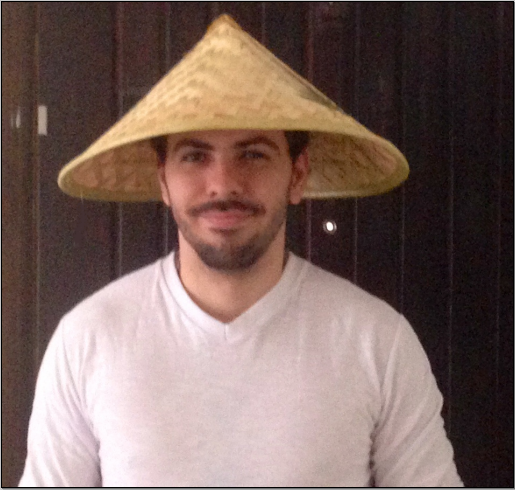
\includegraphics[width=4cm]{images/tony.png}}
  \end{figure}
\end{frame}


\begin{frame}
  \frametitle{Introduction}
  Software Information:
  \begin{itemize}
  \item  Mosca is a Open Source Tool to find bugs
  \item  Mosca held by GPL v3 license: https://github.com/CoolerVoid/Mosca/blob/master/LICENSE.txt
  \end{itemize}
\end{frame}



\begin{frame}
  \frametitle{Introduction}
  Why this tool is made in C language ?
  \begin{itemize}
  \item  C have a high delay time for writing and debugging, but no pain no gain, have a fast performance, addition of this point, the C language is run at any architecture like Mips,ARM and others... at the future can follow mobile implementations. other benefits of C,  have good and high profile to write optimizations, if you think write some lines in ASSEMBLY code with AES-NI or SiMD instructions, i think is good choice. 
  \item  Why you not use POO ? in this project i follow "KISS" principe: http://pt.wikipedia.org/wiki/Keep\_It\_Simple
  \item  C language have a lot old school dudes like a kernel hackers... 
  \end{itemize}
\end{frame}



\begin{frame}
  \frametitle{Introduction}
  Requirements:
  \begin{itemize}
  \item  Need "GCC" and "make", you need pcre library, at linux distributions like debian search package libpcre-dev at RPM distributions search libpcre-devel 
  \item  Current version tested only Unix Like systems(Linux, MacOS and *BSD).
  \item  Current version run well, but is a BeTa version, you can report bug here: https://github.com/CoolerVoid/Mosca/issues
  \end{itemize}
\end{frame}

% \section{Main Body} % add these to see outline in slides

\begin{frame}
  \frametitle{How you can use it}
  Following this to get, decompress, compile and execute:
  \begin{itemize}
  \item wget https://github.com/CoolerVoid/Mosca/archive/master.zip; 
  \item unzip master.zip; cd Mosca-master; make; ./mosca
  \end{itemize}
\end{frame}



\begin{frame}
  \frametitle{The Overview}
  \begin{figure}[]    
    \centering
    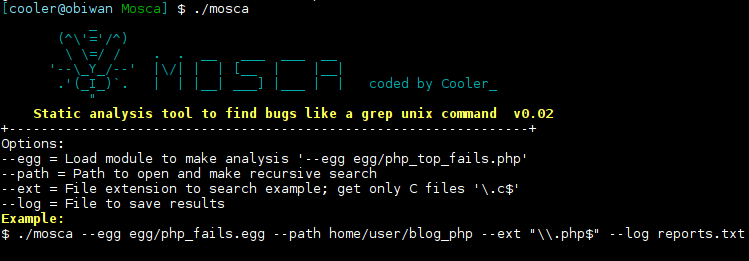
\includegraphics[width=14cm]{images/codeview.png} 
  \end{figure}
\end{frame}


\begin{frame}
  \frametitle{Explain}
  Mosca use Egg Modules
  \begin{itemize}
  \item Each egg is a simple config to find bug at especific language like PHP,Ruby etc...
  \item example of egg config at directory "egg"
  \item If Mosca read a line with vunerability of egg in source code, mosca have alert about and save at logs.
  \end{itemize}
\end{frame}


\begin{frame}
  \frametitle{The End}
  \begin{figure}[]    
    \centering
    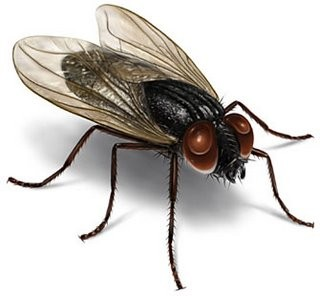
\includegraphics[width=6cm]{images/mosca.jpg} 
  \end{figure}
\end{frame}



% \section{Conclusion} % add these to see outline in slides

\begin{frame}
  \frametitle{Greets}
  \begin{itemize}
  \item IAK, Sigsegv, M0nad, Slyfunky , RaphaelSC, pl4nkton, gustavoRobertux, Muzgo, Otacon...
  \item HB, F-117, Eremita, Clandestine, Loganbr, Geyslan, Clodonil Trigo...
  \item my parents and friends...
  \item https://conviso.com.br/index.php/EN
  \end{itemize}
\end{frame}

\begin{frame}
  \frametitle{at construction...}
\end{frame}

\end{document}
